\documentclass[conference]{IEEEtran}
\IEEEoverridecommandlockouts
% The preceding line is only needed to identify funding in the first footnote. If that is unneeded, please comment it out.
\usepackage{cite}
\usepackage{amsmath,amssymb,amsfonts}
\usepackage{algorithmic}
\usepackage{graphicx}
\usepackage{textcomp}
\usepackage{xcolor}
\usepackage{subcaption}

\def\BibTeX{{\rm B\kern-.05em{\sc i\kern-.025em b}\kern-.08em
    T\kern-.1667em\lower.7ex\hbox{E}\kern-.125emX}}
\begin{document}

\title{ECE276B PR2 Report}

\author{
\IEEEauthorblockN{1\textsuperscript{st} Weixiao Zhan}
\IEEEauthorblockA{
    weixiao-zhan[at]ucsd[dot]edu}
}

\maketitle

\section{Introduction}
Motion planning in robotics involves determining a policy or a path 
from a certain start state to a certain goal state 
while minimizing the cost and avoiding obstacles. 
This project focuses on solving a deterministic motion planning problem in 
3-D Euclidean space with axis-aligned bounding boxes (AABB) obstacles
using search-based and sample-based algorithms. 

Search-based algorithms systematically explore the state space to find a path, 
while sample-based algorithms randomly sample the space and connect samples to construct a feasible path. 
Specifically, this project implements collision checking for AABB, 
A* algorithm, probabilistic road map (PRM), rapidly exploring random tree (RRT), and RRT*. 
Lastly, evaluations are made between search-based and sampling-based methods.


\section{Problem Formulation}
The deterministic motion planning problem can be described as the collection of 
state space $\mathcal{X}$, control space $\mathcal{U}$, motion model $f$, time horizon $T$
stage cost $l$, and terminal cost $q$.
Denote the start state as $s$ and the goal state as $\tau$.

\subsection{State Space}
In this project, the environment is a collection of one boundary AABB (denote as $B$) 
and $m$ obstacle AABBs (denote as $O_i$). 
Each AABB represents a set of points within a box-shaped range. \
An AABB can be compactly parameterized by two $\mathbb{R}^3$ points, 
i.e., the lower left $l$ and the top right $r$:

\[
\begin{aligned}
    \text{env} &= \{B, O_1, O_2, \cdots, O_m \in \text{AABB}\} \\
    \text{AABB}_{l,r} &= \left\{ p \middle| \begin{gathered}
    l, p, r \in \mathbb{R}^{3} \\
    l_{i} \leq p_{i} \leq r_{i}, i \in \{x, y, z\}
    \end{gathered} \right\}
\end{aligned}
\]

The state space is all free space in the environment:
\[
\mathcal{X} = \left\{ p \middle| p \in \left( B \setminus \bigcup_i O_i \right) \right\}
\]

Due to the limited numerical precision on computers, 
the search-based planner must explicitly discretize the state space. 
Denote the discretization scale as $\phi$, that is, discretize 1 unit of each axis into $\phi$ cells.
All points within each cell are considered the same and located at the center of the cell.
The sample-based planner only consider a finite sampled subset of state space.
$$
\begin{aligned}
    \mathcal{X}_{search} &= \left\{ \text{int}(\phi p), \forall p \in \mathcal{X} \right\} \\
    \mathcal{X}_{sample} &\subset \mathcal{X}
\end{aligned}
$$

\subsection{Control Space}
In search-based planning, 
the point can move in all diagonal directions, 
allowing for 26 possible moves from each state. 
Whereas in sample-based planning, the point can move any length in any direction.

\[
\begin{aligned}
    \mathcal{U}_{\text{search}} &= \left\{ -\frac{1}{\phi}, 0, \frac{1}{\phi} \right\}^{3} \\ 
    \mathcal{U}_{\text{sample}} &= \mathbb{R}^{3}
\end{aligned}
\]

\subsection{Motion Model}
The motion model is deterministic.
\[
f(x, u) = x + u \quad \text{iff} \quad x + u \in \mathcal{X}
\]

\subsection{Stage Cost and Terminal Cost}
\[
\begin{aligned}
    l(x, u) &= \| u \|_{2} \\
    q(x) &= \begin{cases} 
        0 & x = \text{goal} \\ 
        \infty & \text{otherwise}
    \end{cases}
\end{aligned}
\]

\subsection{Equivalent Shortest Path Problem}
The deterministic motion planning problem is equivalent to the shortest path problem. 
Thus, finding an optimal control policy is equivalent to 
finding the shortest path in a certain graph $G$:

\[
\begin{aligned}
G_{\Lambda} &= \left\{
\begin{aligned}
    V &= \mathcal{X}_{\Lambda} \\ 
    E &= \left\{ (x \rightarrow f(x,u)) \middle| 
        \begin{gathered}
            \forall x \in \mathcal{X}_{\Lambda} \\
            \forall u \in \mathcal{U}_{\Lambda} 
        \end{gathered}
        \right\} 
\end{aligned}
\right\} \\
\Lambda &= search, sample
\end{aligned}
\]

Given a shortest path $(s \rightarrow p_1 \rightarrow \cdots p_i \rightarrow \cdots\tau)$,
the corresponding optimal control policy is 
$$\pi_{T-i}(p_i) = p_{i+1} - p_{i}$$


\section{Technical Approach}

\subsection{Collision Checking Environment Class}
The \texttt{CollisionCheckingEnvironment} class is 
the framework for representing the environment and the state space.
It implemented following primitives:

\subsubsection{\texttt{load}}
load environment from text file and apply discretization if desired.

\subsubsection{\texttt{point\_collide}}
checks whether a point locate inside any obstacles or outside the boundary.
The method is cached using LRU-cache decorator to improve performance by avoiding redundant checks,
especially in search-based planner.

\subsubsection{\texttt{line\_collide}}
checks whether a line segment collides with any obstacles.
This is achieved using the \texttt{trimesh} library:
each AABB obstacle is converted to a 3-D mesh composed of 12 triangles;
the line segment is converted to a ray;
and ray tracing is used to find intersections.
Then, the intersections are checked whether lying on the line segment.

Note if a line segment compactly lies within one obstacle, 
this method will not report collision.
Thus, \texttt{point\_collide} need to be used in conjunction 
to ensure entire line segment lies in free space.

\subsubsection{\texttt{sample\_free}}
sample random points in the environment's free space.

\subsubsection{visualization}
Additionally, the class includes visualization functions
to render the environment with obstacles, start, and goal points, 
aiding in visual debugging and analysis.

\subsection{Search-Based Planner}
The \texttt{SearchBasedPlanner} class provides an abstract framework for 
implementing label correcting algorithm in a 3-D environment. 
It maintains:
\begin{itemize}
    \item \texttt{start} and \texttt{goal}: The start and goal positions in the environment.
    \item \texttt{g}: A dictionary to hold the cost from the start to each node, initialized to infinity.
    \item \texttt{parent}: A dictionary to hold the shortest path tree, mapping each node to its parent.
    \item \texttt{open\_list}: A set containing the frontier nodes during the search.
    \item \texttt{close\_set}: A set to keep track of expanded nodes.
\end{itemize}
and support:
\begin{itemize}
    \item \texttt{iter\_children}: generates valid (no collision) child nodes (neighbors) and their respective stage costs.
    \item \texttt{build\_path}: reconstructs the path from the goal to the start using the parent pointers, computing the total path cost.
\end{itemize}
All search-based implementation only need to overload the \texttt{search} method.

\subsubsection{A*}
inherits from \texttt{SearchBasedPlanner} and implements the A* algorithm.
The heuristic function used is the L2 norm (Euclidean distance), which is also cached for efficiency. 
The \texttt{open\_list} is revised to a priority queue sorted by $g + heuristic$.

Its \texttt{search} method initializes the cost to the start node 
and inserts it into the open list with its heuristic value. 
The main loop iteratively expands the node with the lowest estimated total cost until the goal is reached. 
During expansion, it updates the cost and parent for each valid child node 
and adds them to the open list if a shorter path is found.

\subsection{Sample-Based Planner}
The \texttt{SampleBasedPlanner} class provides an abstract framework for implementing sample-based motion planning algorithms in a 3-D environment. It maintains:
\begin{itemize}
    \item \texttt{start} and \texttt{goal}: The start and goal positions in the environment.
    \item \texttt{radius}: The critical radius
    $$r^* = 2\left( 1+\frac{1}{d}  \right)^{\frac{1}{d} } \left( \frac{Vol(C_{free})}{Vol(Unit-ball)}  \right)^{\frac{1}{d} } \left( \frac{\log \left( n \right) }{n}  \right)^{\frac{1}{d} } $$
    \item \texttt{graph}: A \texttt{networkx} graph to represent the sampled nodes and edges.
\end{itemize}
and supports:
\begin{itemize}
    \item \texttt{build\_path}: Search shortest path from start to goal 
    using \texttt{networkX} build in dijkstra algorithm.
    \item \texttt{near} and \texttt{nearest}: Finds near nodes of a given node
    using \texttt{cKDTree} from \texttt{sk-lean} library to accelerate computation.
    \item \texttt{steer}: Generates a point that steers from the start towards the goal by a specified distance.
\end{itemize}
All sample-based implementation only need to overload the \texttt{sample} method.

\subsubsection{PRM}
inherits from \texttt{SampleBasedPlanner}. 
Its \texttt{sample} method generates a roadmap by 
randomly sampling nodes in the free space and 
connecting new nodes to their nearby nodes if the path between them is collision-free. 

\subsubsection{RRT}
inherits from \texttt{SampleBasedPlanner} and revise the \texttt{graph} to a directed graph. 
Its \texttt{sample} method generate a tree by 
randomly sampling nodes in the free space and
connecting new nodes to their nearest node if the path between them is collision-free.
Every certain period, RRT will try to connect the goal with nearest node on the tree.

\subsubsection{RRT*}
extends \texttt{RRT} with optimal capabilities. 
It maintains a cost dictionary to track the cost to each node from the start. 
Its \texttt{sample} method, in addition to the routine in RRT's \texttt{sample},
also rewire the tree in the local region around the new node if there is a better path to nearby nodes via the new node.
After rewiring, the cost reduction is cascade to all descendant of the rewired near node.

\section{Results}

Five planner are compared: A* ($\phi = 5, 8$),
PRM, RRT, RRT* (first path and final path).
For A*, two discretization scale are used and compared.
For sample-based planner,
the radius is set to critical radius $r^*$;
the number of iteration is set to terminate 
when the graph had $N = 2000$ valid nodes;
the steer step is set to 0.2.
For RRT*, both the first path and final path are reported.

\subsection{quality of path}
Figure \ref{fig:path-length} illustrates the shortest path lengths found 
by various planner across different environments. 
The RRT and RRT* algorithms failed to find any valid path in the "monza" environment 
within a reasonable (50,000) iterations due to the special construction of the environment, 
which will be discussed in a later section.

A* planner with larger discretization scale and finer path granularity can
produce slightly shorter paths. 

A* and other Search-based planners are limited to 45-degree movements,
thus, despite explored all nodes systematically, 
their result is not the true shortest path.
In face, sample-based planners can sometimes produce slightly shorter path than A*.

Among sample-based planners, 
the standard RRT produces the longest paths. 
Whereas, PRM and RRT* can find equally good paths compared to search-based planners.
In addition, RRT* can continue to improve the path quality with more iterations and rewiring.

\begin{figure*}[h]
    \centering
    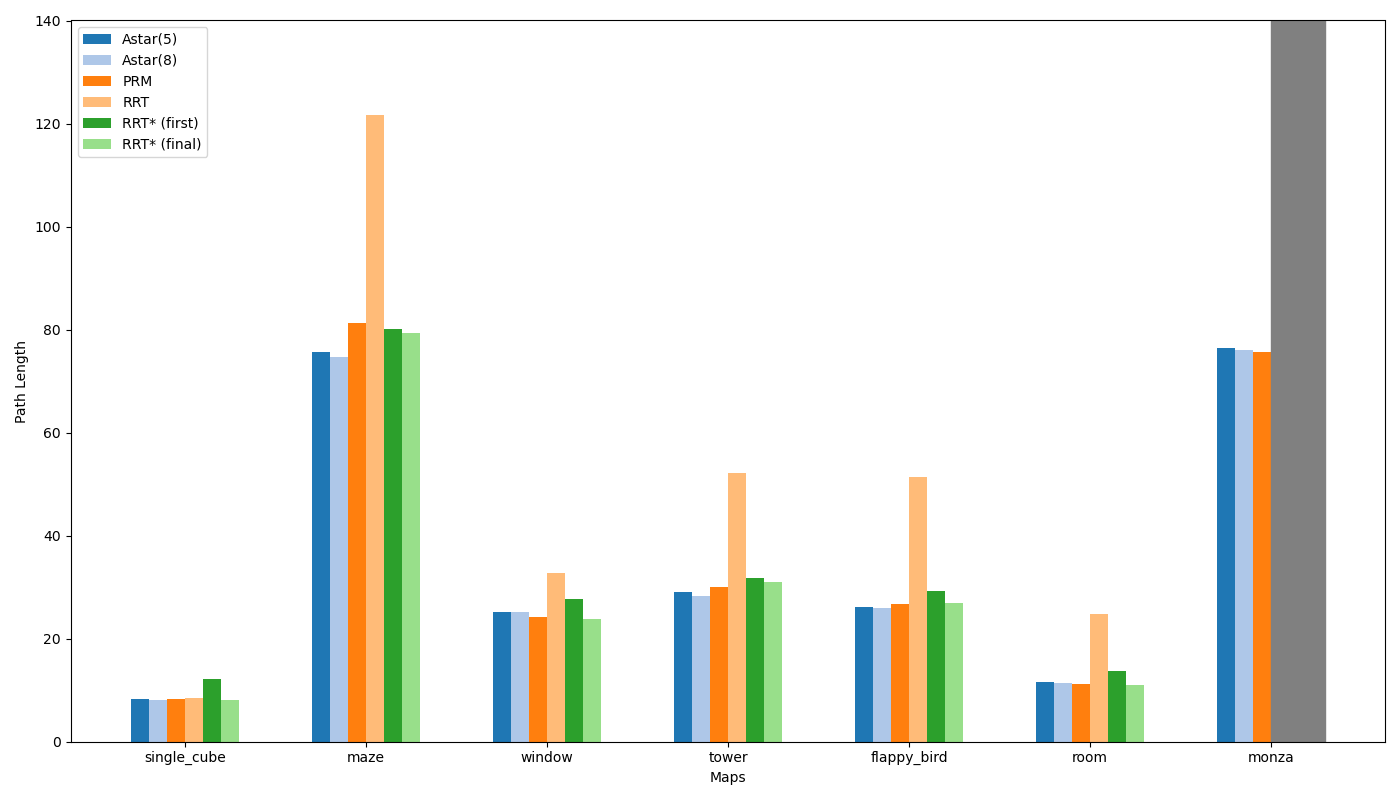
\includegraphics[width=\linewidth]{img/path_length.png}
    \caption{Path Length Comparison}
    \label{fig:path-length}
\end{figure*}


\subsection{Runtime and Solution Size}
The time complexity and memory complexity is measured by 
the total runtime (shown in Figure \ref{fig:runtime}) and
the size of solution (shown in Figure \ref{fig:sol-size}) respectively.

The size of solution
% represented by the number of nodes or edges been considered to produce the result,
is defined to as:
\begin{enumerate}
    \item A*: the number of nodes in open and close set;
    \item PRM: the number of edges in graph. 
    Note: the PRM always iterates $N$ times and produce a graph with $N$ nodes.
    \item RRT and RRT*: the number of sample iteration to build the $N$ node tree. 
    Note: not every iteration in RRT and RRT* can add new nodes to the graph.
    Thus, the solution size is measured in number of sample iterations.
\end{enumerate}

Based on Figure \ref{fig:runtime} and \ref{fig:sol-size},
when the l2 heuristic works well, such as "single cube" and "room" environment,
A* planner is the fastest and uses the fewest memory.
However, when the heuristic doesn't work well, such as "maze" environment,
A* planner is the slowest and uses significantly more memory. 
Moreover, any slightly increment in discretization scale would case the solution size cubically increase in worse case.

For PRM planner, the number edge stays largely the same 
across different environments.

\begin{figure*}
    \centering
    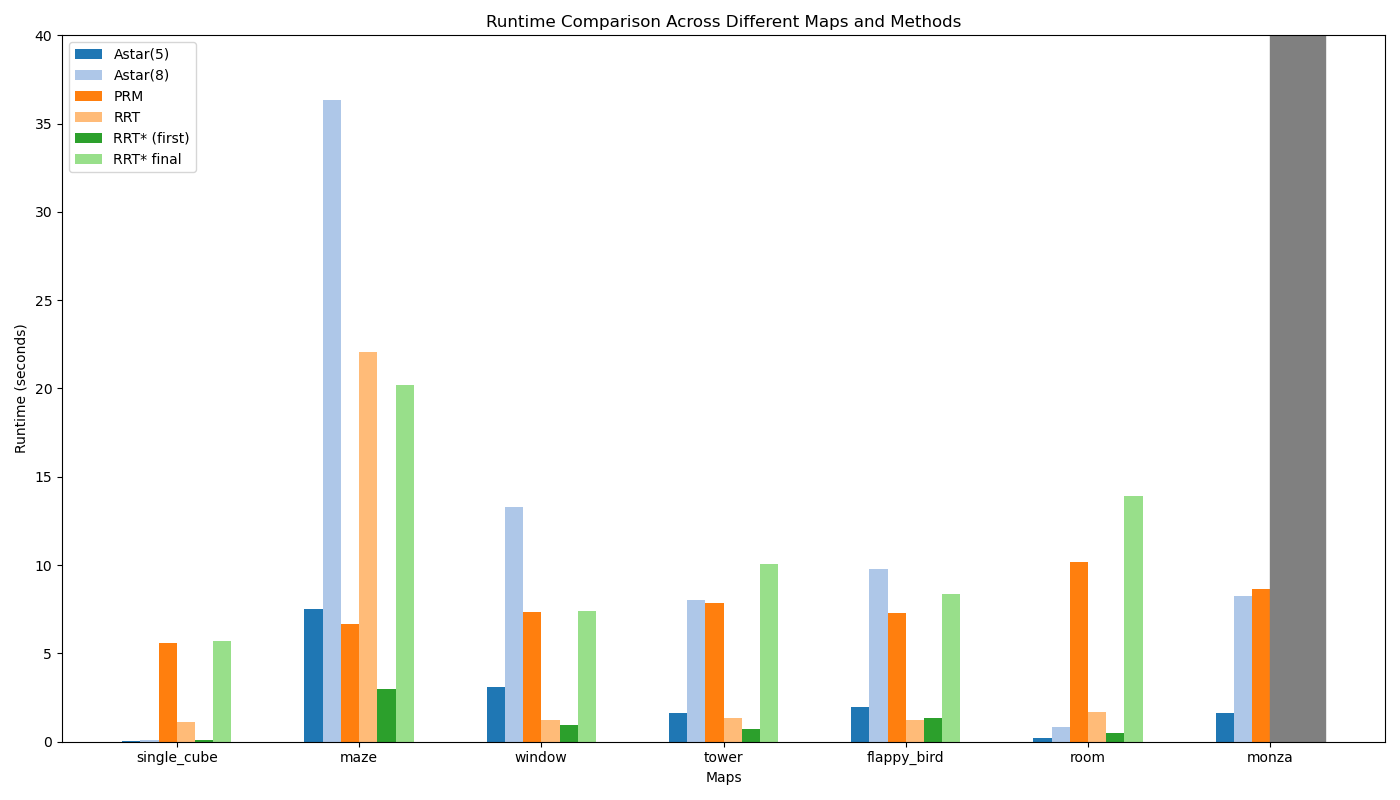
\includegraphics[width=\linewidth]{img/runtime.png}
    \caption{Runtime}
    \label{fig:runtime}
\end{figure*}

\begin{figure*}
    \centering
    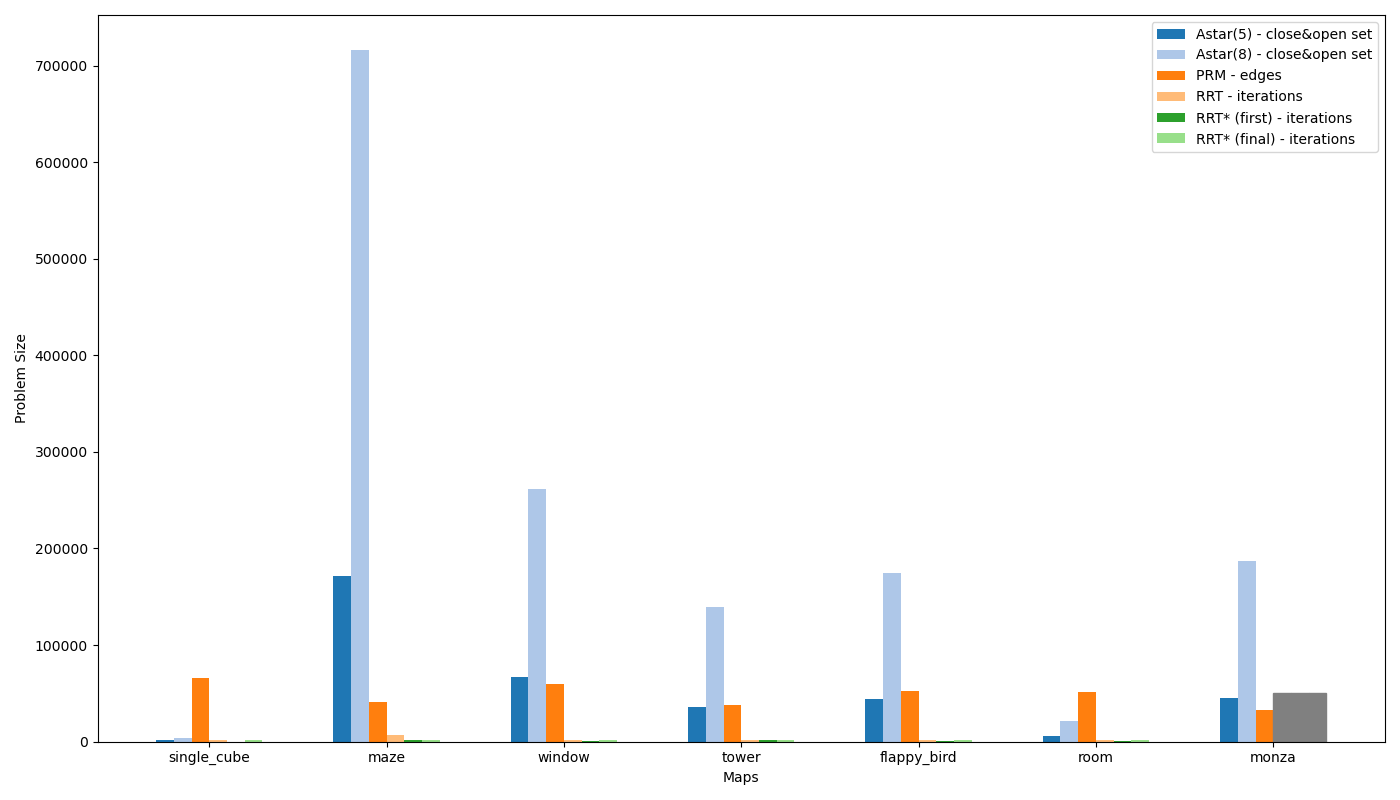
\includegraphics[width=\linewidth]{img/problem_size.png}
    \caption{Solution Size}
    \label{fig:sol-size}
\end{figure*}

\subsection{profiling}
\texttt{cProfile} library is used to further investigate program profile of A* and PRM planner.
Figure \ref{fig:profile} shows that 
A* spend most of its time on iterating child nodes and compute hashes for indexing.
Where as PRM spend most of its time on collision checking.

\begin{figure*}
    \centering
    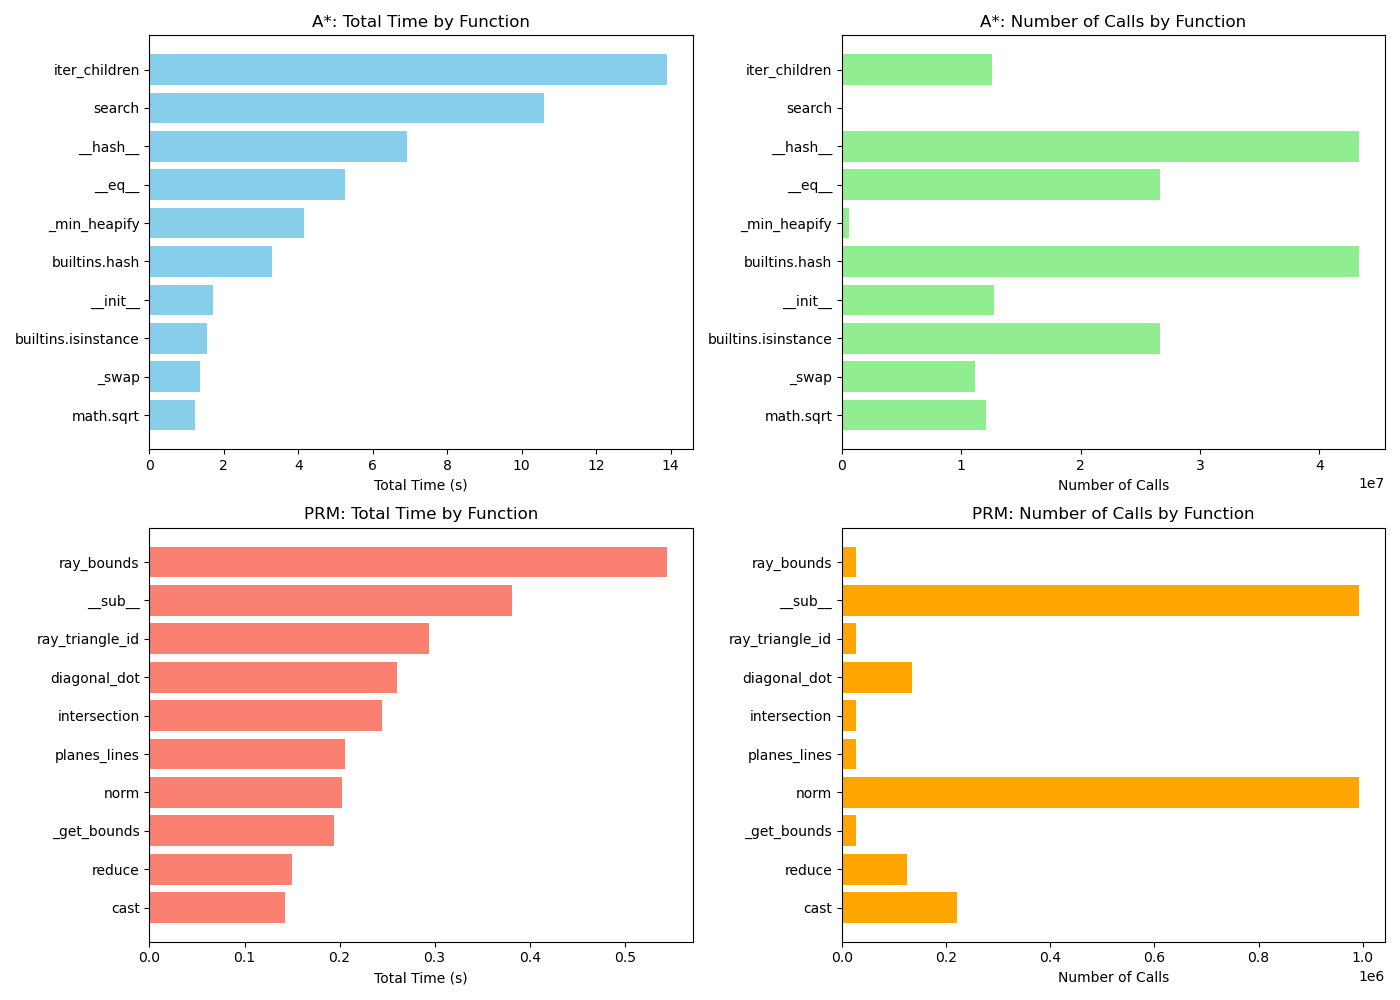
\includegraphics[width=0.8\linewidth]{img/profile.png}
    \caption{Profile}
    \label{fig:profile}
\end{figure*}

\subsection{PRM vs RRT}
Shown in  Figure \ref{fig:runtime} and \ref{fig:sol-size},
RRT runs faster and consume fewer memory than PRM.
However, this comes with the cost of less robust and more sensitive 
to the environment layout.

Figure \ref{fig:monza} shows the PRM and RRT on monza environment 
after $\frac{N}{2} = 1000$ iterations.
The PRM is already able to expand though the entire free space and connect to the goal.
Where as the RRT is stuck behind the first wall.

RRT only try to connect the nearest point.
Since the wall is skinny, 
most of the nearest nodes will lay on two side of the wall.
Their connection attempt would fail due to collision checking.
Thus RRT is struggle to make progress in such environment construction.

On the other hand, PRM always add the new node into graph in every iterations.
The new node may not connect to the graph imminently, 
but they are place holders to support future new nodes and improvements.

\begin{figure*}[htbp]
    \centering
    \begin{subfigure}[b]{0.45\linewidth}
        \centering
        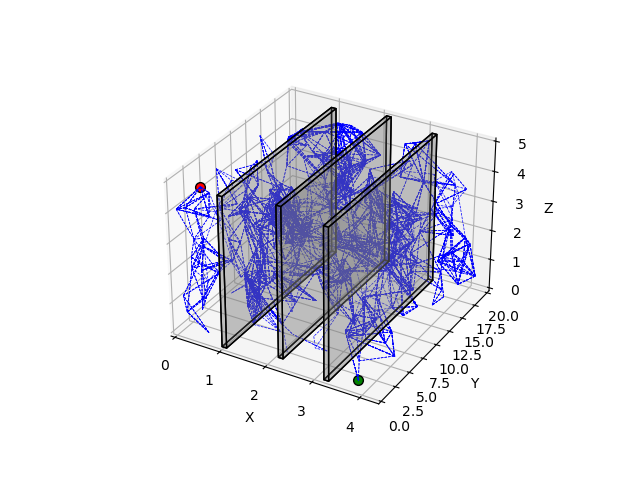
\includegraphics[width=\linewidth]{img/monza-PRM.png}
        \caption{PRM after $\frac{N}{2}$ iterations}
        \label{fig:monza-PRM}
    \end{subfigure}
    \begin{subfigure}[b]{0.45\linewidth}
        \centering
        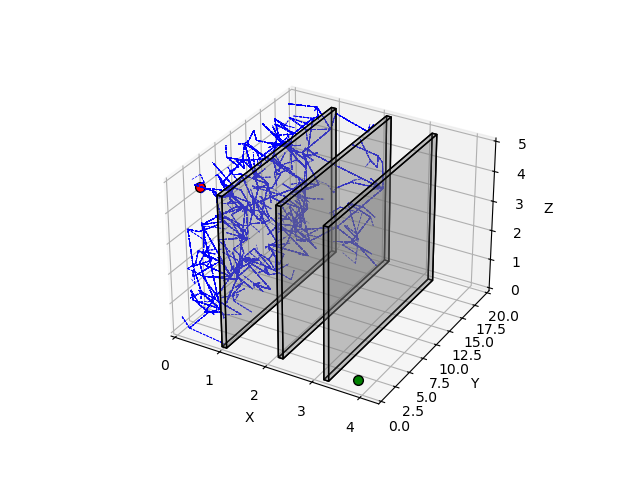
\includegraphics[width=\linewidth]{img/monza-RRT.png}
        \caption{RRT after $\frac{N}{2}$ iterations}
        \label{fig:monza-RRT}
    \end{subfigure}
    \caption{Monza environment}
    \label{fig:monza}
\end{figure*}


\subsection{RRT vs RRT*: rewire effect}
Figure \ref{fig:sc} shows RRT and RRT* in single cube environment
after $\frac{N}{2} = 1000$ iterations.
The rewiring in RRT* is able to revise the randomly generated 
tree into radial shape, representing the optimal path from start to any sampled nodes.

\begin{figure*}[htbp]
    \centering
    \begin{subfigure}[b]{0.45\linewidth}
        \centering
        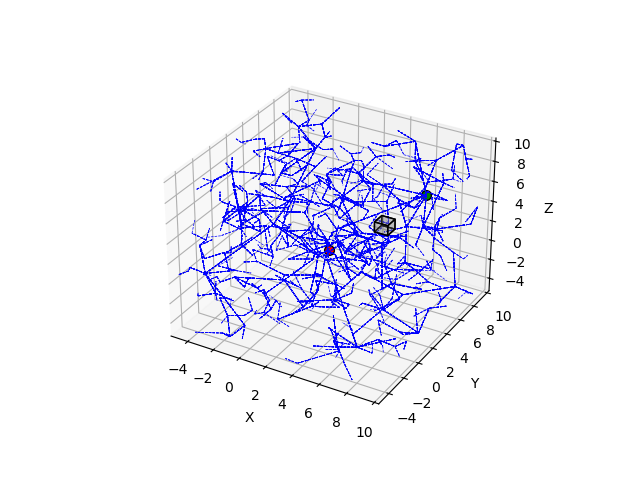
\includegraphics[width=\linewidth]{img/sc-RRT.png}
        \caption{RRT after $\frac{N}{2}$ iterations}
        \label{fig:sc-RRT}
    \end{subfigure}
    \begin{subfigure}[b]{0.45\linewidth}
        \centering
        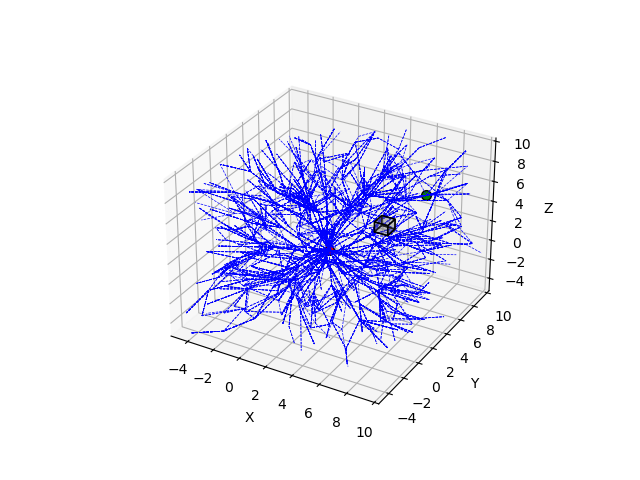
\includegraphics[width=\linewidth]{img/sc-RRT*.png}
        \caption{RRT* after $\frac{N}{2}$ iterations}
        \label{fig:sc-RRT*}
    \end{subfigure}
    \caption{Single cube environment}
    \label{fig:sc}
\end{figure*}

In summary, 
A* rely on good heuristic function to work well.
PRM is probabilistically optimal and most robust among sample-based planners. 
but it is slow to compute and consume much memory.
RRT reduces the runtime and memory footprint, but is less robust and not probabilistically optimal.
RRT* introduced rewiring step to achieved probabilistically optimal but the runtime is slow down to PRM level.

\appendix
Shortest path of all methods in all environment is shown in Figure \ref{fig:environments}.
For interactive result, run \texttt{plot.py}

\begin{figure*}[htbp]
    \centering

    \begin{subfigure}[b]{0.3\textwidth}
        \centering
        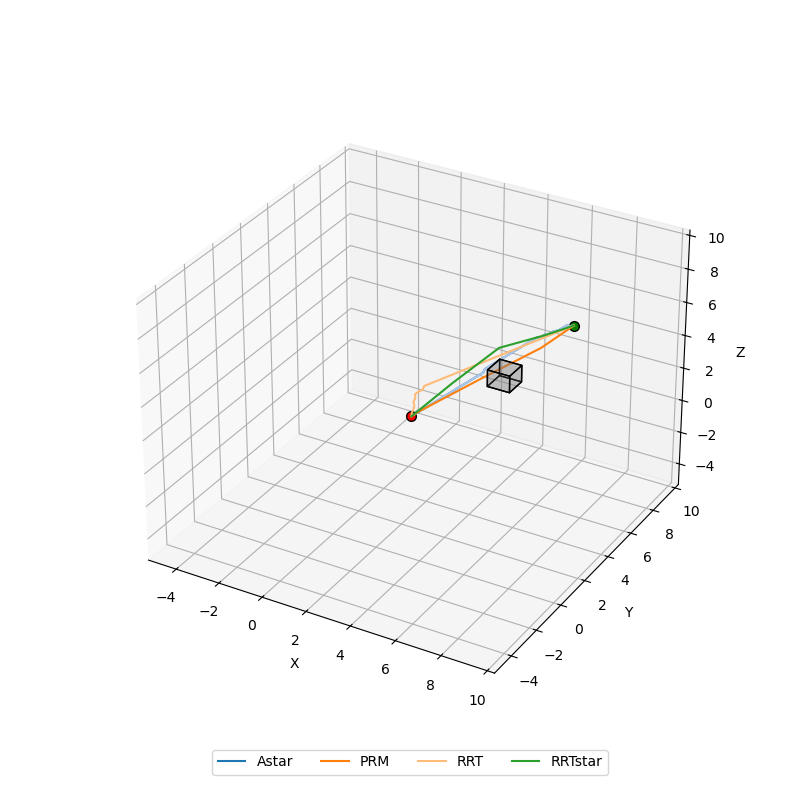
\includegraphics[width=\textwidth]{img/single_cube.png}
        \caption{Single Cube}
    \end{subfigure}
    \hfill
    \begin{subfigure}[b]{0.3\textwidth}
        \centering
        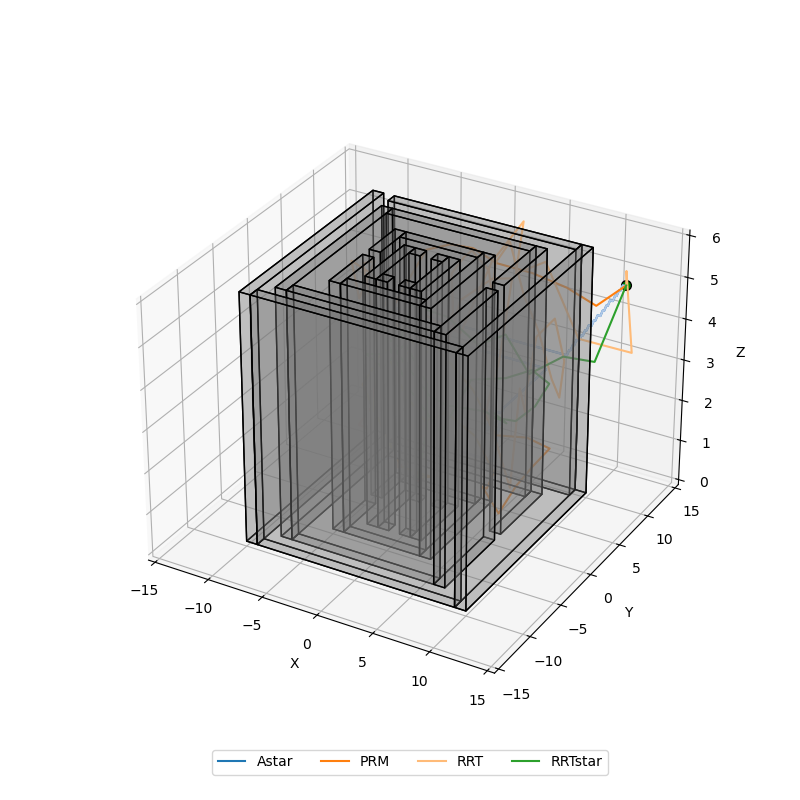
\includegraphics[width=\textwidth]{img/maze.png}
        \caption{Maze}
    \end{subfigure}
    \hfill
    \begin{subfigure}[b]{0.3\textwidth}
        \centering
        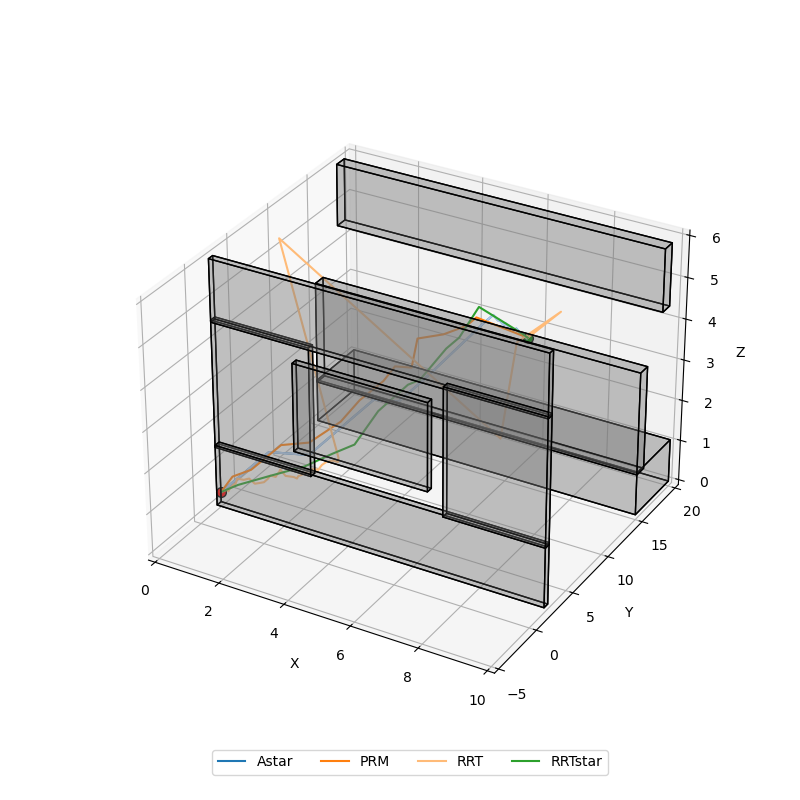
\includegraphics[width=\textwidth]{img/window.png}
        \caption{Window}
    \end{subfigure}

    \vskip\baselineskip

    \begin{subfigure}[b]{0.3\textwidth}
        \centering
        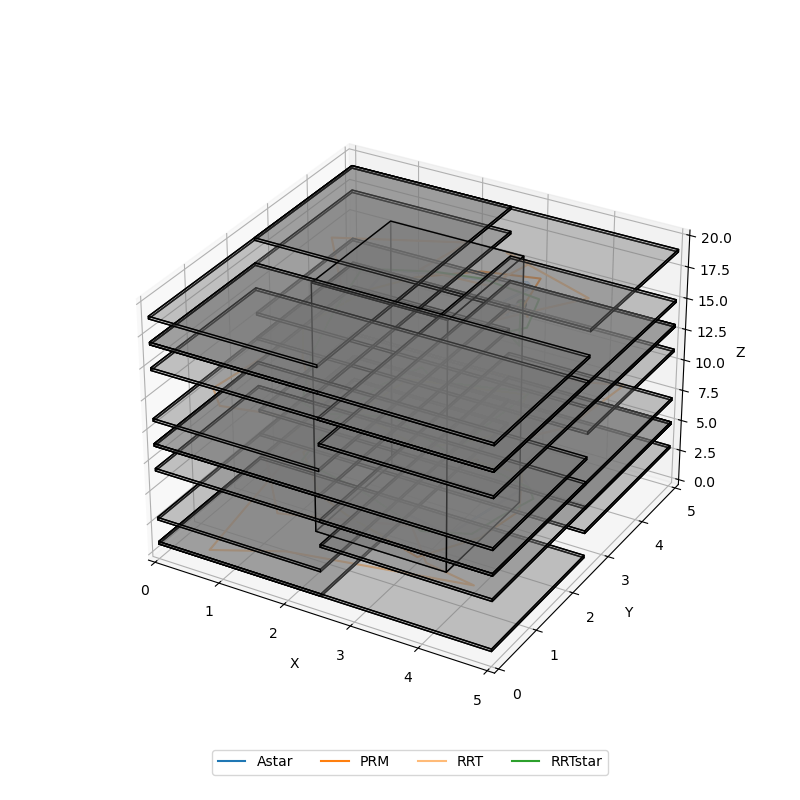
\includegraphics[width=\textwidth]{img/tower.png}
        \caption{Tower}
    \end{subfigure}
    \hfill
    \begin{subfigure}[b]{0.3\textwidth}
        \centering
        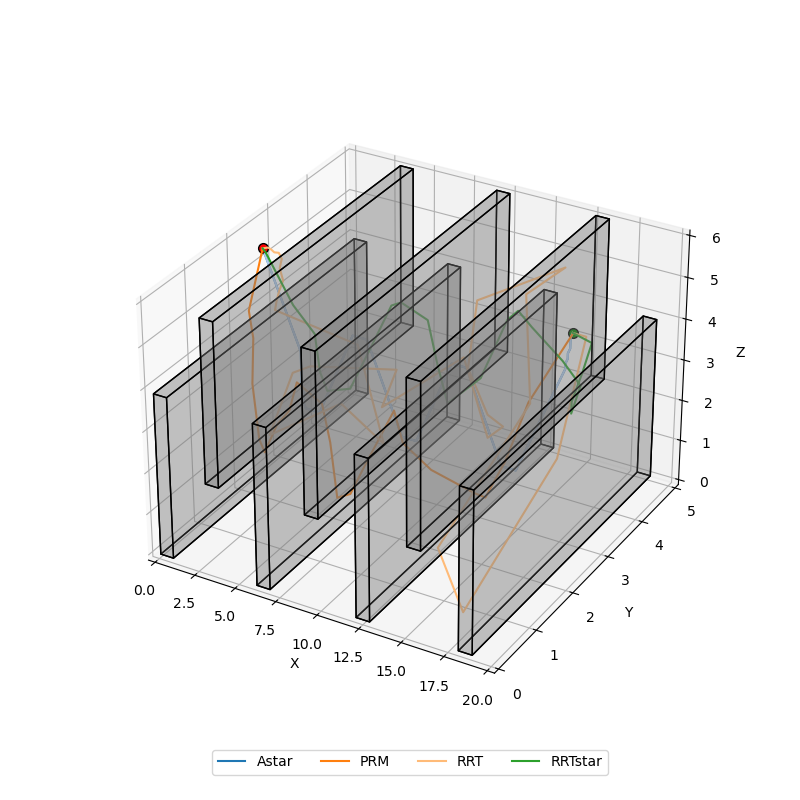
\includegraphics[width=\textwidth]{img/flappy_bird.png}
        \caption{Flappy Bird}
    \end{subfigure}
    \hfill
    \begin{subfigure}[b]{0.3\textwidth}
        \centering
        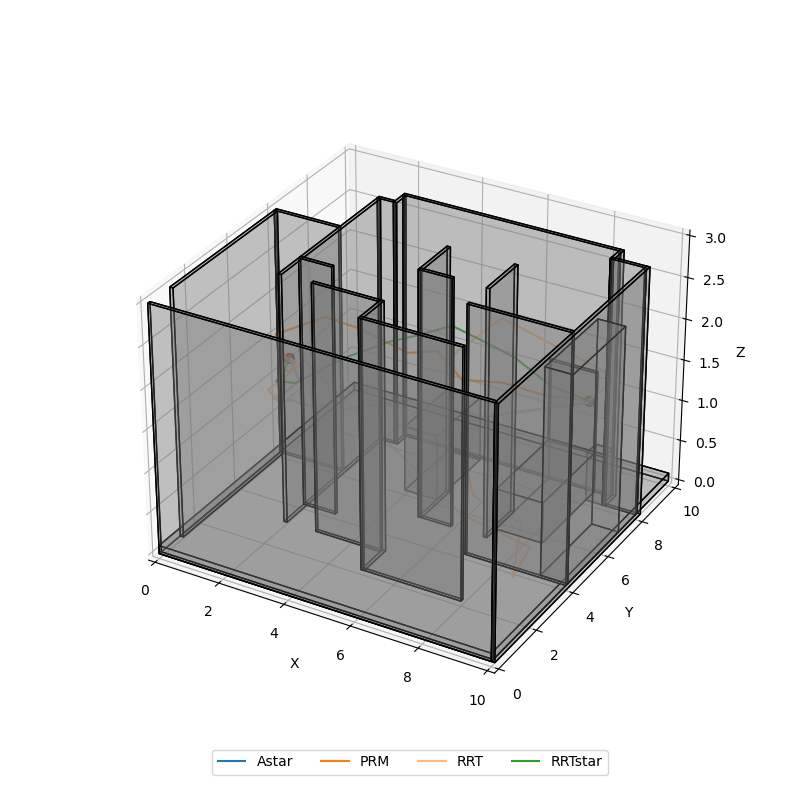
\includegraphics[width=\textwidth]{img/room.png}
        \caption{Room}
    \end{subfigure}

    \vskip\baselineskip

    \begin{subfigure}[b]{0.3\textwidth}
        \centering
        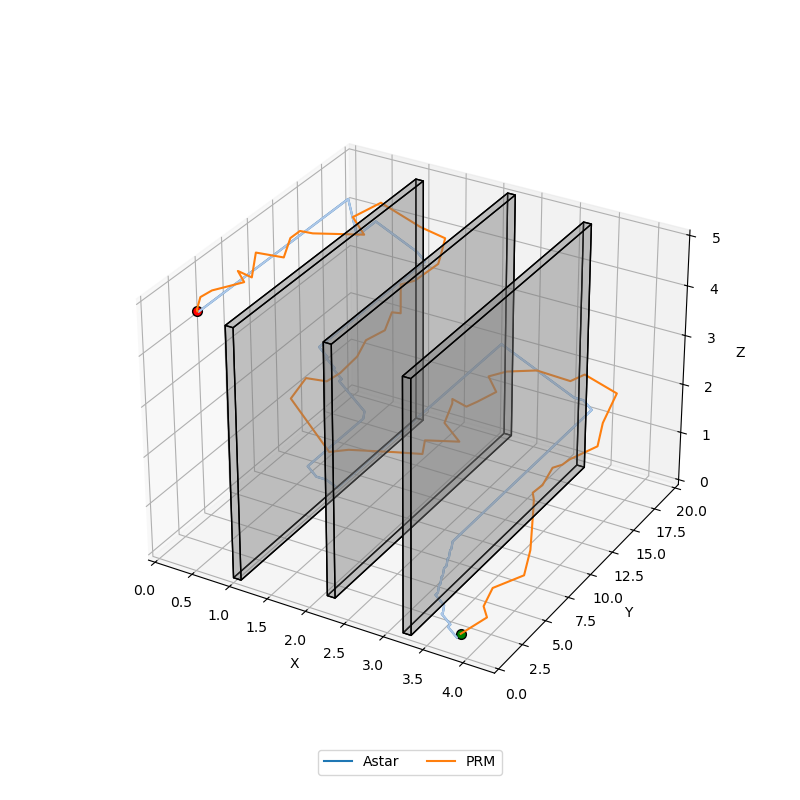
\includegraphics[width=\textwidth]{img/monza.png}
        \caption{Monza}
    \end{subfigure}

    \caption{hortest path of all methods in all environment}
    \label{fig:environments}
\end{figure*}

\end{document}
